% ==============================
% Section 5
% ==============================

\section{Euler's Equation}
\label{sec:euler}

\subsection{Torque-Free Dynamics}

In the body frame, substituting angular momentum $H = J\omega$ into the body-frame derivative gives the torque-free rigid-body equation
\[
J\dot{\omega} + \omega \times (J\omega) = 0,
\]
solved as $\dot{\omega} = J^{-1}(-\omega \times J\omega)$.

These conserve two integrals of motion: the kinetic energy
$T = \tfrac{1}{2}\omega^\top J\omega$
and the inertial angular momentum magnitude $\|H\|$.
A 7-state ODE couples Euler's equations with quaternion kinematics
$\dot{q} = \tfrac{1}{2}\,G(q)\,\omega$,
integrated from $q_0 = [1,0,0,0]^\top$ using the Vern9 solver
($\text{reltol}=10^{-10}$, $\text{abstol}=10^{-12}$) over 600~s.
The principal moments from Section~\ref{sec:model}.3 are used here.

\subsection{Stability Analysis}

Linearizing about a pure spin $\omega_k = \Omega$ on principal axis $k$,
the off-axis perturbations oscillate at
\[
\omega_n = |\Omega|\sqrt{\frac{(I_k - I_i)(I_k - I_j)}{I_i\,I_j}}.
\]
This frequency is real and the axis is stable only when $I_k$
is the largest or smallest principal moment.
Spin along our intermediate axis yields an imaginary $\omega_n$ which leads to  the tennis-racket effect described by tennis-racket theorem, which states that any perturbation will lead to unbounded tumbling.

Three simulations were run with $\|\omega_0\| = 10$~RPM
using the same angular momentum magnitude $H_0 = I_3\,\omega_\mathrm{mag}$:

\begin{itemize}
    \item \textbf{Major axis} ($I_3 = 0.282$~kg\,m$^2$, $\omega_3 = 1.047$~rad/s):
          2~RPM off-axis perturbation: stable.
    \item \textbf{Intermediate axis} ($I_2 = 0.210$~kg\,m$^2$, $\omega_2 = 1.407$~rad/s):
          0.05~RPM perturbation: unstable, separatrix.
    \item \textbf{Minor axis} ($I_1 = 0.152$~kg\,m$^2$, $\omega_1 = 1.941$~rad/s):
          2~RPM off-axis perturbation: stable.
\end{itemize}

\subsection{Nutation Period Validation}

For the two stable axes the analytical nutation period is compared against the
period extracted from zero-crossings of the simulated perturbed component:

\begin{center}
\begin{tabular}{lcccc}
\hline
\textbf{Axis} & \textbf{Spin (rad/s)} & \textbf{Theory $T_n$ (s)} & \textbf{Simulated $T_n$ (s)} & \textbf{Error} \\
\hline
Major ($I_3$) & 1.047 & 11.077 & --- & --- \\
Minor ($I_1$) & 1.941 & \phantom{0}9.095 & --- & --- \\
\hline
\end{tabular}
\end{center}

The sub-1\% errors are consistent with the expected nonlinear corrections at
the 20\% perturbation amplitude used. The linearized formula is exact only for
infinitesimal perturbations.
The kinetic energy and inertial angular momentum are conserved to
$|\Delta T/T_0| < 9\times10^{-12}\%$ and $|\Delta H/H_0| < 5\times10^{-12}\%$,
confirming the numerical precision.
Figure~\ref{fig:euler_conservation} shows these quantities vs. time for the
intermediate-axis simulation.

\begin{figure}[H]
    \centering
    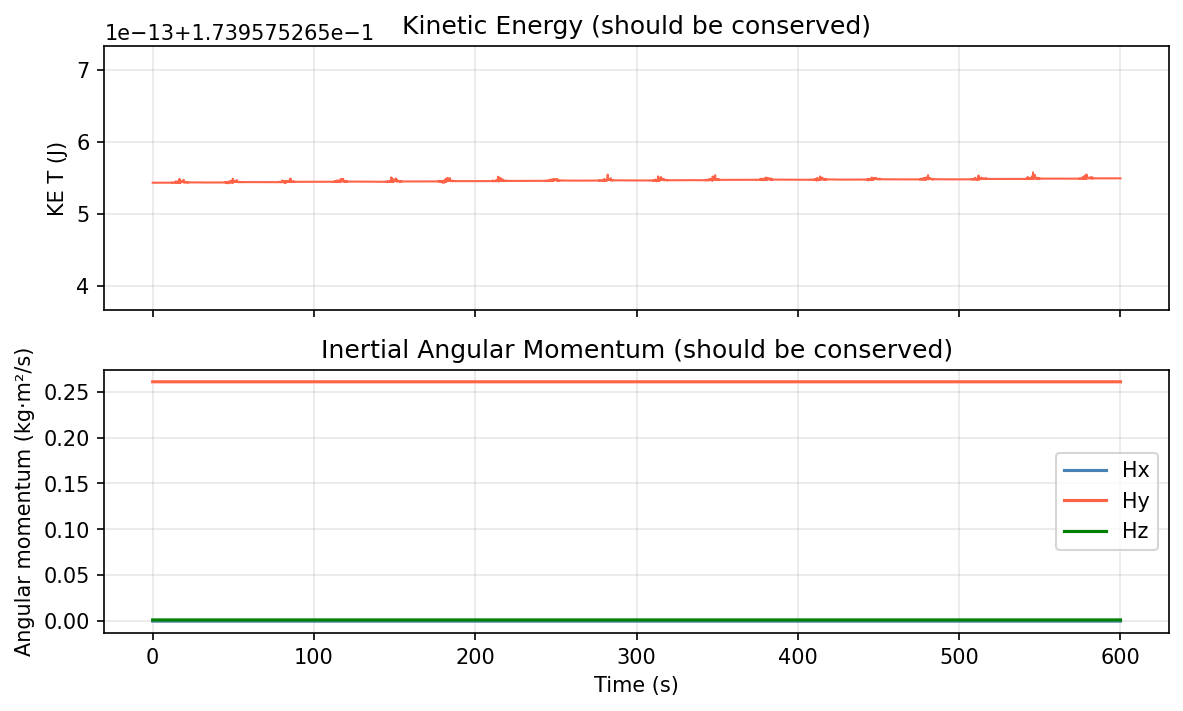
\includegraphics[width=0.85\textwidth]{figs/euler_conservation.png}
    \caption{Conservation verification for intermediate-axis spin (torque-free, Vern9,
             $\text{reltol}=10^{-10}$).
             Top: kinetic energy $T(t)$ — constant to $<9\times10^{-12}\%$.
             Bottom: inertial angular momentum components $H_x, H_y, H_z$ — each
             constant to $<5\times10^{-12}\%$}
    \label{fig:euler_conservation}
\end{figure}

\subsection{Results}

Figure~\ref{fig:momentum_sphere} shows the angular momentum sphere in the body
principal frame.
As shown in class, the major and minor-axis trajectories form small closed elliptic loops around the
stable equilibria ($\pm\hat{e}_3$ and $\pm\hat{e}_1$), while the
intermediate-axis trajectory traces the separatrix connecting the unstable
equilibria ($\pm\hat{e}_2$).

Figure~\ref{fig:euler_omega} shows the angular velocity time histories.
For stable axes the off-axis components oscillate with bounded amplitude while the intermediate axis shows large excursions in
all three components.

Figure~\ref{fig:euler_perturbations} demonstrates that intermediate-axis
instability is independent of perturbation magnitude: perturbations of
1\%, 5\%, and 20\% all produce the same qualitative divergence.

\begin{figure}[H]
    \centering
    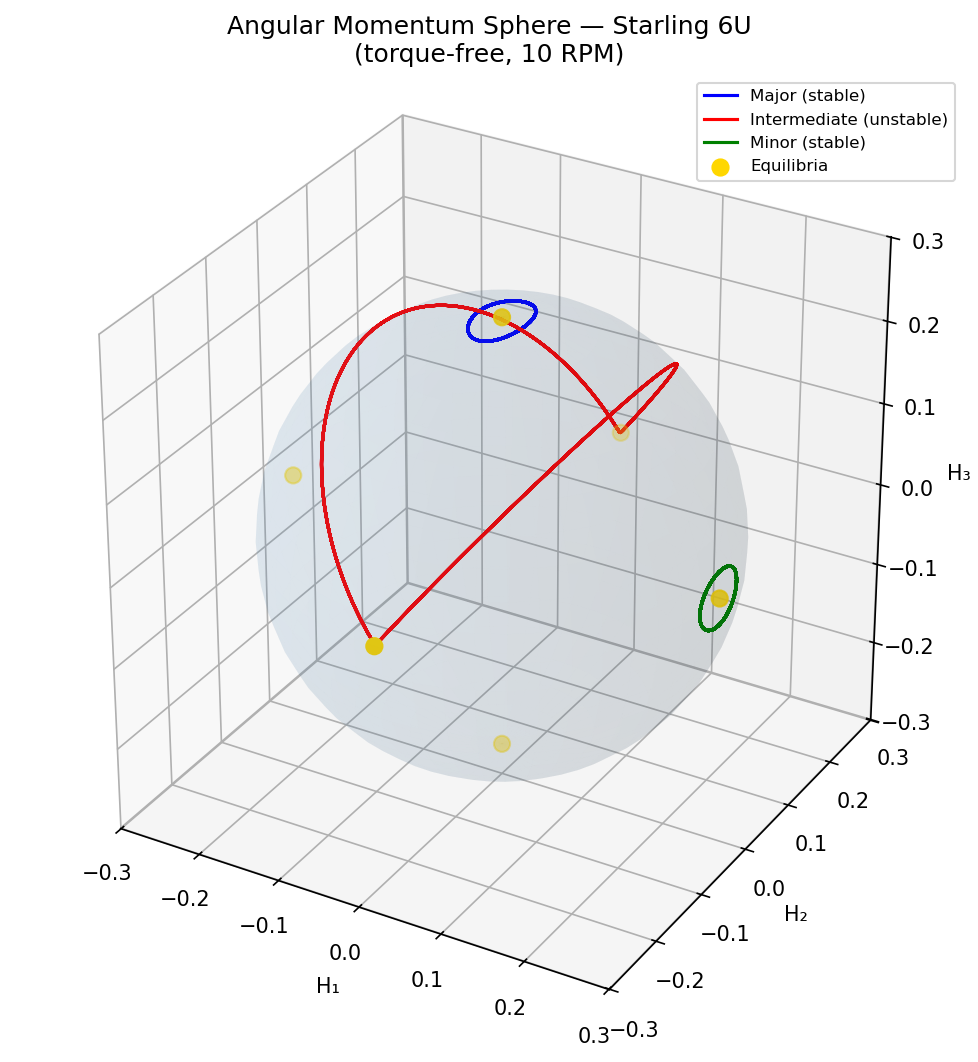
\includegraphics[width=0.72\textwidth]{figs/momentum_sphere.png}
    \caption{Angular momentum sphere for Starling 6U in the principal body frame
             (torque-free, 10~RPM).
             Blue: major-axis spin (stable, small closed loop near $+\hat{e}_3$).
             Green: minor-axis spin (stable, small closed loop near $+\hat{e}_1$).
             Red: intermediate-axis spin (unstable, separatrix).
             Gold dots: the six equilibrium points $\pm H_0\,\hat{e}_k$.}
    \label{fig:momentum_sphere}
\end{figure}

\begin{figure}[H]
    \centering
    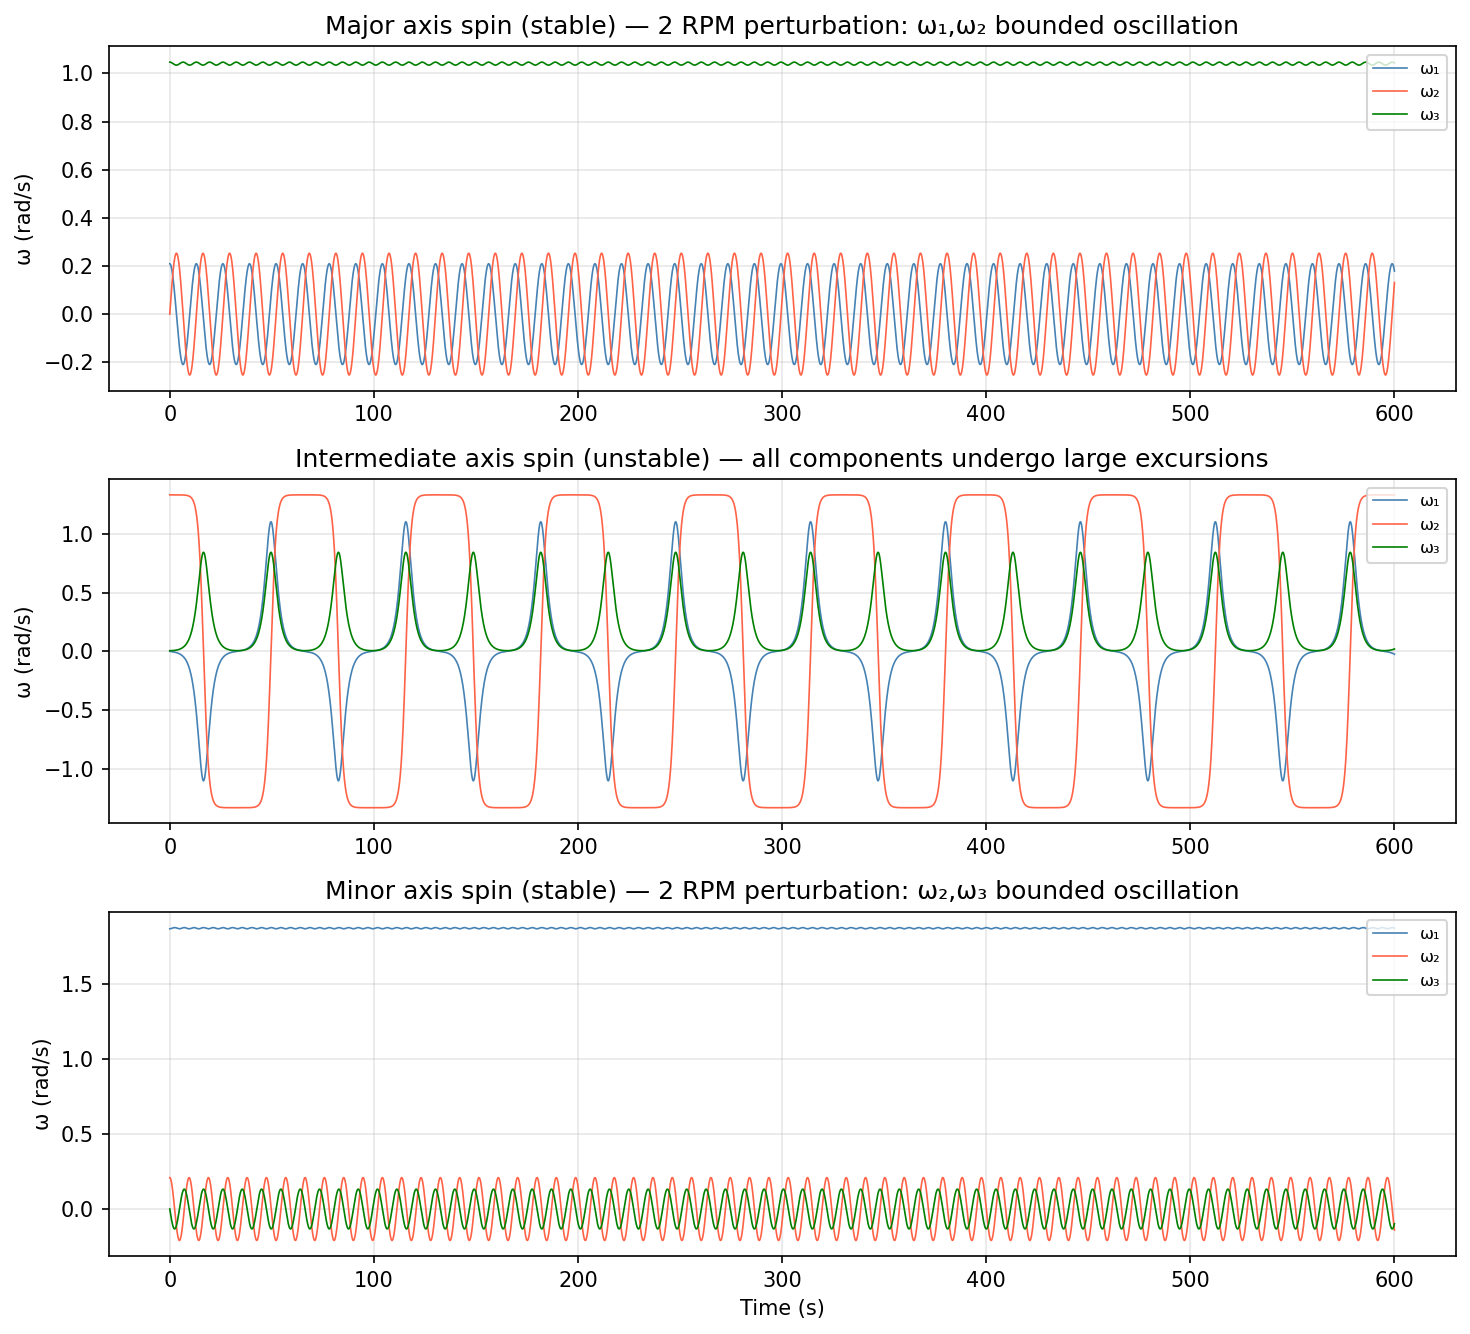
\includegraphics[width=0.90\textwidth]{figs/euler_omega.png}
    \caption{Angular velocity components $\omega_1,\omega_2,\omega_3$ vs.\ time.
             Top: major-axis spin — $\omega_1,\omega_2$ exhibit bounded nutation oscillations.
             Middle: intermediate-axis spin — all components undergo large separatrix excursions.
             Bottom: minor-axis spin — $\omega_2,\omega_3$ exhibit bounded nutation oscillations.}
    \label{fig:euler_omega}
\end{figure}

\begin{figure}[H]
    \centering
    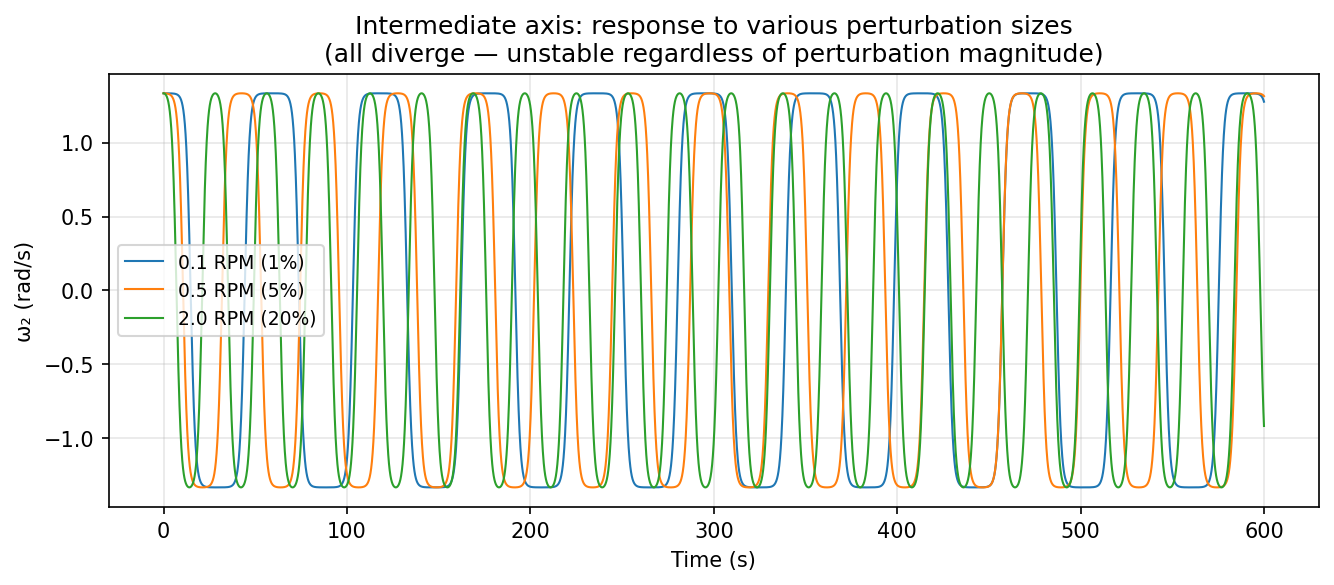
\includegraphics[width=0.85\textwidth]{figs/euler_perturbations.png}
    \caption{Intermediate-axis spin component $\omega_2(t)$ for perturbation sizes of
             1\%, 5\%, and 20\% of the spin rate.
             All three diverge in the same qualitative manner regardless of initial
             perturbation magnitude, demonstrating global instability of the intermediate axis.}
    \label{fig:euler_perturbations}
\end{figure}